\documentclass[11pt, a4paper]{article}

% --- packages ---
\usepackage[utf8]{inputenc}
\usepackage[T1]{fontenc}
\usepackage{lmodern}
\usepackage[margin=2.5cm]{geometry}
\usepackage{amsmath, amssymb}
\usepackage{booktabs}
\usepackage{graphicx}
\usepackage{hyperref}
\usepackage{xcolor}
\usepackage{caption}
\usepackage{float}
\usepackage{enumitem}
\usepackage{microtype}
\usepackage{parskip}

\hypersetup{
    colorlinks=true,
    linkcolor=blue!60!black,
    citecolor=blue!60!black,
    urlcolor=blue!60!black,
}

\title{%
    \textbf{Discrete Goalpost Widening} \\[0.4em]
    \large How Pity Cap Manipulation Extends the Uncertainty Window \\
    to Maximise Spending Pressure in Gacha Loot Systems
}

% Suppress author and date blocks entirely.
\author{\vspace{-2em}}
\date{\vspace{-2em}}

\begin{document}
\maketitle

\begin{abstract}
    This paper presents a Monte Carlo analysis of the Sanctum loot
    system, synthesising two independent findings to expose the
    monetisation function of the S1 pity cap. A Shapley-value variance
    decomposition reveals that S1 timing dominates outcome uncertainty
    in the critical early-to-mid session (accounting for up to 68.9\%
    of explained variance at roll~50). A parameter sweep across pity
    caps from 10 to 80 rolls shows that each 10-roll increment extends
    the zone of peak uncertainty by 11--14 rolls. The synthesis
    demonstrates that the current 80-roll cap places the \emph{entire}
    uncertainty window over both player archetypes: casual players
    who exit at the 150-point redemption threshold (roll~$\sim$38)
    and skin-seekers who commit to the pity cap for the max prize
    (roll~80). For casual players, only 16.5\% trigger the pity
    guarantee by their exit point; the cap functions as a
    psychological anchor rather than a practical mechanic. For
    skin-seekers, the cap sets the price of the guaranteed outcome
    at \pounds214 rather than the \pounds85--\pounds108 it would
    cost at caps of 30--40. The cumulative effect of widening the
    cap from 10 to 80 rolls generates 79 additional anxious rolls,
    representing \pounds213 in potential additional spend per player.
\end{abstract}

\tableofcontents
\newpage


% ======================================================================
\section{Introduction and Motivation}
\label{sec:intro}
% ======================================================================

Gacha loot systems are a dominant monetisation strategy in
free-to-play games, generating revenue through randomised item
acquisition. A core design element in many such systems is the
\emph{pity mechanic}: a guaranteed high-value outcome after a
specified number of unsuccessful rolls. The pity cap is typically
presented to players as a consumer-friendly safeguard --- a ceiling
on bad luck. This paper examines whether the cap also serves a
second, less visible function: as a precision tool for calibrating
spending pressure.

The Sanctum loot system awards items from a pool of 753 possibilities
distributed across three subsets:
\begin{itemize}[nosep]
    \item \textbf{Subset~1 (S1):} 1 one-time item + 1 permanent item,
          total selection probability 0.50\%. The one-time S1 item is
          the highest-value outcome, and its acquisition triggers a
          \emph{transform} that permanently alters the probability
          distribution. Pity guarantees this transform within $N$ rolls
          (default $N = 80$).
    \item \textbf{Subset~2 (S2):} 10 one-time items + 1 permanent item,
          total probability 10.00\%.
    \item \textbf{Subset~3 (S3):} 742 items (5 permanent + 263 emotes +
          474 icons), total probability 89.50\%.
\end{itemize}

Each roll selects one item according to a probability distribution
that evolves dynamically: one-time items are removed after collection,
and their probability mass is redistributed among remaining items
within the same subset. The mathematical foundations of this process
--- two-stage sampling, inverse CDF sampling, and probability
redistribution --- are detailed in the companion document
\texttt{simulation\_foundations.pdf}.

The central question of this paper is: \emph{how does varying the S1
pity cap affect both the statistical properties of player outcomes
and the psychological conditions under which spending decisions are
made?}

This is addressed by connecting two independent analyses:
\begin{enumerate}[nosep]
    \item A \textbf{Shapley-value variance decomposition} that
          quantifies how much of the total outcome variance is
          attributable to S1 timing, S2 timing, and S3 item selection
          at each roll.
    \item A \textbf{pity cap parameter sweep} that measures expected
          point accumulation, variance, and rolls-to-target across
          caps from 10 to 80 in increments of 10.
\end{enumerate}

The synthesis of these two findings reveals the mechanism termed
\emph{discrete goalpost widening}: incremental cap increases that
each appear modest in isolation but cumulatively extend the zone of
maximum outcome uncertainty across the player's entire natural session.


% ======================================================================
\section{Method}
\label{sec:method}
% ======================================================================

All simulations use 300{,}000 independent trials of up to 1{,}000
rolls each, executed on an NVIDIA GeForce RTX 5060~Ti via CuPy for
GPU-accelerated computation. The random seed is fixed at 42 for
reproducibility. Full implementation details are in
\texttt{expected\_points.py}.

\subsection{Variance Decomposition}
\label{sec:method-variance}

The total variance of cumulative points at each roll is decomposed
into contributions from three sources of randomness:

\begin{itemize}[nosep]
    \item \textbf{S1 timing:} when the S1 transform occurs.
    \item \textbf{S2 timing:} when all S2 one-time items are collected.
    \item \textbf{S3 selection:} which specific S3 items are drawn on
          each roll.
\end{itemize}

Following a $2^3$ factorial design, eight simulation configurations
are run: a baseline with all sources free, three single-fix variants
(each fixing one source at its baseline median), three double-fix
variants, and a fully-fixed variant. The contribution of each source
is computed via Shapley values, which account for interaction effects
by averaging marginal contributions across all possible orderings.

Formally, for source $i$, the Shapley value is:
\begin{equation}
    \phi_i = \sum_{S \subseteq \{1,2,3\} \setminus \{i\}}
    \frac{|S|!\,(2 - |S|)!}{3!}
    \left[ V(S \cup \{i\}) - V(S) \right]
\end{equation}
where $V(S)$ denotes the variance reduction when the sources in $S$
are fixed. This ensures the decomposition is unique, symmetric, and
sums to the total explained variance.

A sensitivity analysis confirms that the decomposition is robust to
the choice of fix-point: results are stable across the 25th, 50th,
and 75th percentile trigger rolls for both S1 and S2.

\subsection{Pity Cap Parameter Sweep}
\label{sec:method-sweep}

The S1 pity cap is swept across
$\{10, 20, 30, 40, 50, 60, 70, 80\}$ rolls, running 300{,}000
simulations at each value. For each configuration, the following are
recorded:

\begin{itemize}[nosep]
    \item Mean and median cumulative points at checkpoint rolls
          (10, 20, 30, 50, 80, 100, 250).
    \item Standard deviation per roll.
    \item The fraction of simulations that have triggered S1 by each
          roll.
    \item Median rolls required to reach point targets
          (50, 100, 150, 200, 300, 500 points).
\end{itemize}

\subsection{Synthesis: The Uncertainty Window}
\label{sec:method-synthesis}

The synthesis phase connects both analyses by measuring S1's variance
contribution \emph{at each pity cap}. For each cap value, a baseline
simulation and a fix-S1 variant (forcing S1 to trigger at its median
roll for that cap) are run. S1's variance share at roll $r$ is:
\begin{equation}
    \text{S1 share}(r) = \frac{V_{\text{baseline}}(r) - V_{\text{fix-S1}}(r)}{V_{\text{baseline}}(r)}
\end{equation}

The \textbf{uncertainty window} is defined as the contiguous roll
range where S1's smoothed variance share exceeds 30\% (using a
10-roll moving average). This threshold captures the zone where a
single binary event --- whether S1 has triggered --- accounts for
nearly a third or more of all outcome variation.


% ======================================================================
\section{Results}
\label{sec:results}
% ======================================================================

\subsection{S1 Timing Dominates Early-to-Mid Session Variance}
\label{sec:results-variance}

The Shapley decomposition reveals a clear pattern: S1 timing is the
dominant source of outcome uncertainty throughout the critical
early-to-mid game, despite S1 items comprising only 0.5\% of the
probability mass.

\begin{table}[H]
\centering
\caption{Shapley variance decomposition at the default pity cap
(80 rolls). $V_{\text{total}}$ is baseline variance; percentages
are shares of explained variance
($V_{\text{total}} - V_{\text{residual}}$).}
\label{tab:shapley}
\begin{tabular}{r r r r r r r}
\toprule
Roll & $V_{\text{total}}$ & $V_{\text{residual}}$ & S1 & S2 & S3 & Sum \\
\midrule
10   & 253       & 27       & 28.4\% & 0.0\%  & 71.6\% & 100.0\% \\
25   & 952       & 46       & 51.2\% & 0.6\%  & 48.2\% & 100.0\% \\
50   & 2{,}903   & 97       & 68.9\% & 0.4\%  & 30.7\% & 100.0\% \\
100  & 20{,}951  & 11{,}911 & 55.6\% & 25.9\% & 18.5\% & 100.0\% \\
250  & 44{,}774  & 32{,}624 & 47.7\% & 17.8\% & 34.5\% & 100.0\% \\
\bottomrule
\end{tabular}
\end{table}

At roll 25 --- roughly where many players are actively engaged ---
S1 timing accounts for 51.2\% of explained variance. By roll 50 this
rises to 68.9\%. The implication is stark: the single most important
factor determining whether a player's session feels ``lucky'' or
``unlucky'' is whether S1 has triggered.

Critically, the interaction effects from the $2^3$ factorial
analysis confirm that S1 timing acts nearly independently of S2 and
S3. All two-way and three-way interaction terms are below 1.5\% of
baseline variance at every checkpoint. This independence means the
pity cap is a \emph{clean, isolated lever}: adjusting it modifies
spending pressure without creating unpredictable knock-on effects
elsewhere in the system.

% --- Figure: Variance decomposition ---
% Uncomment and adjust path when plots are available:
% \begin{figure}[H]
%     \centering
%     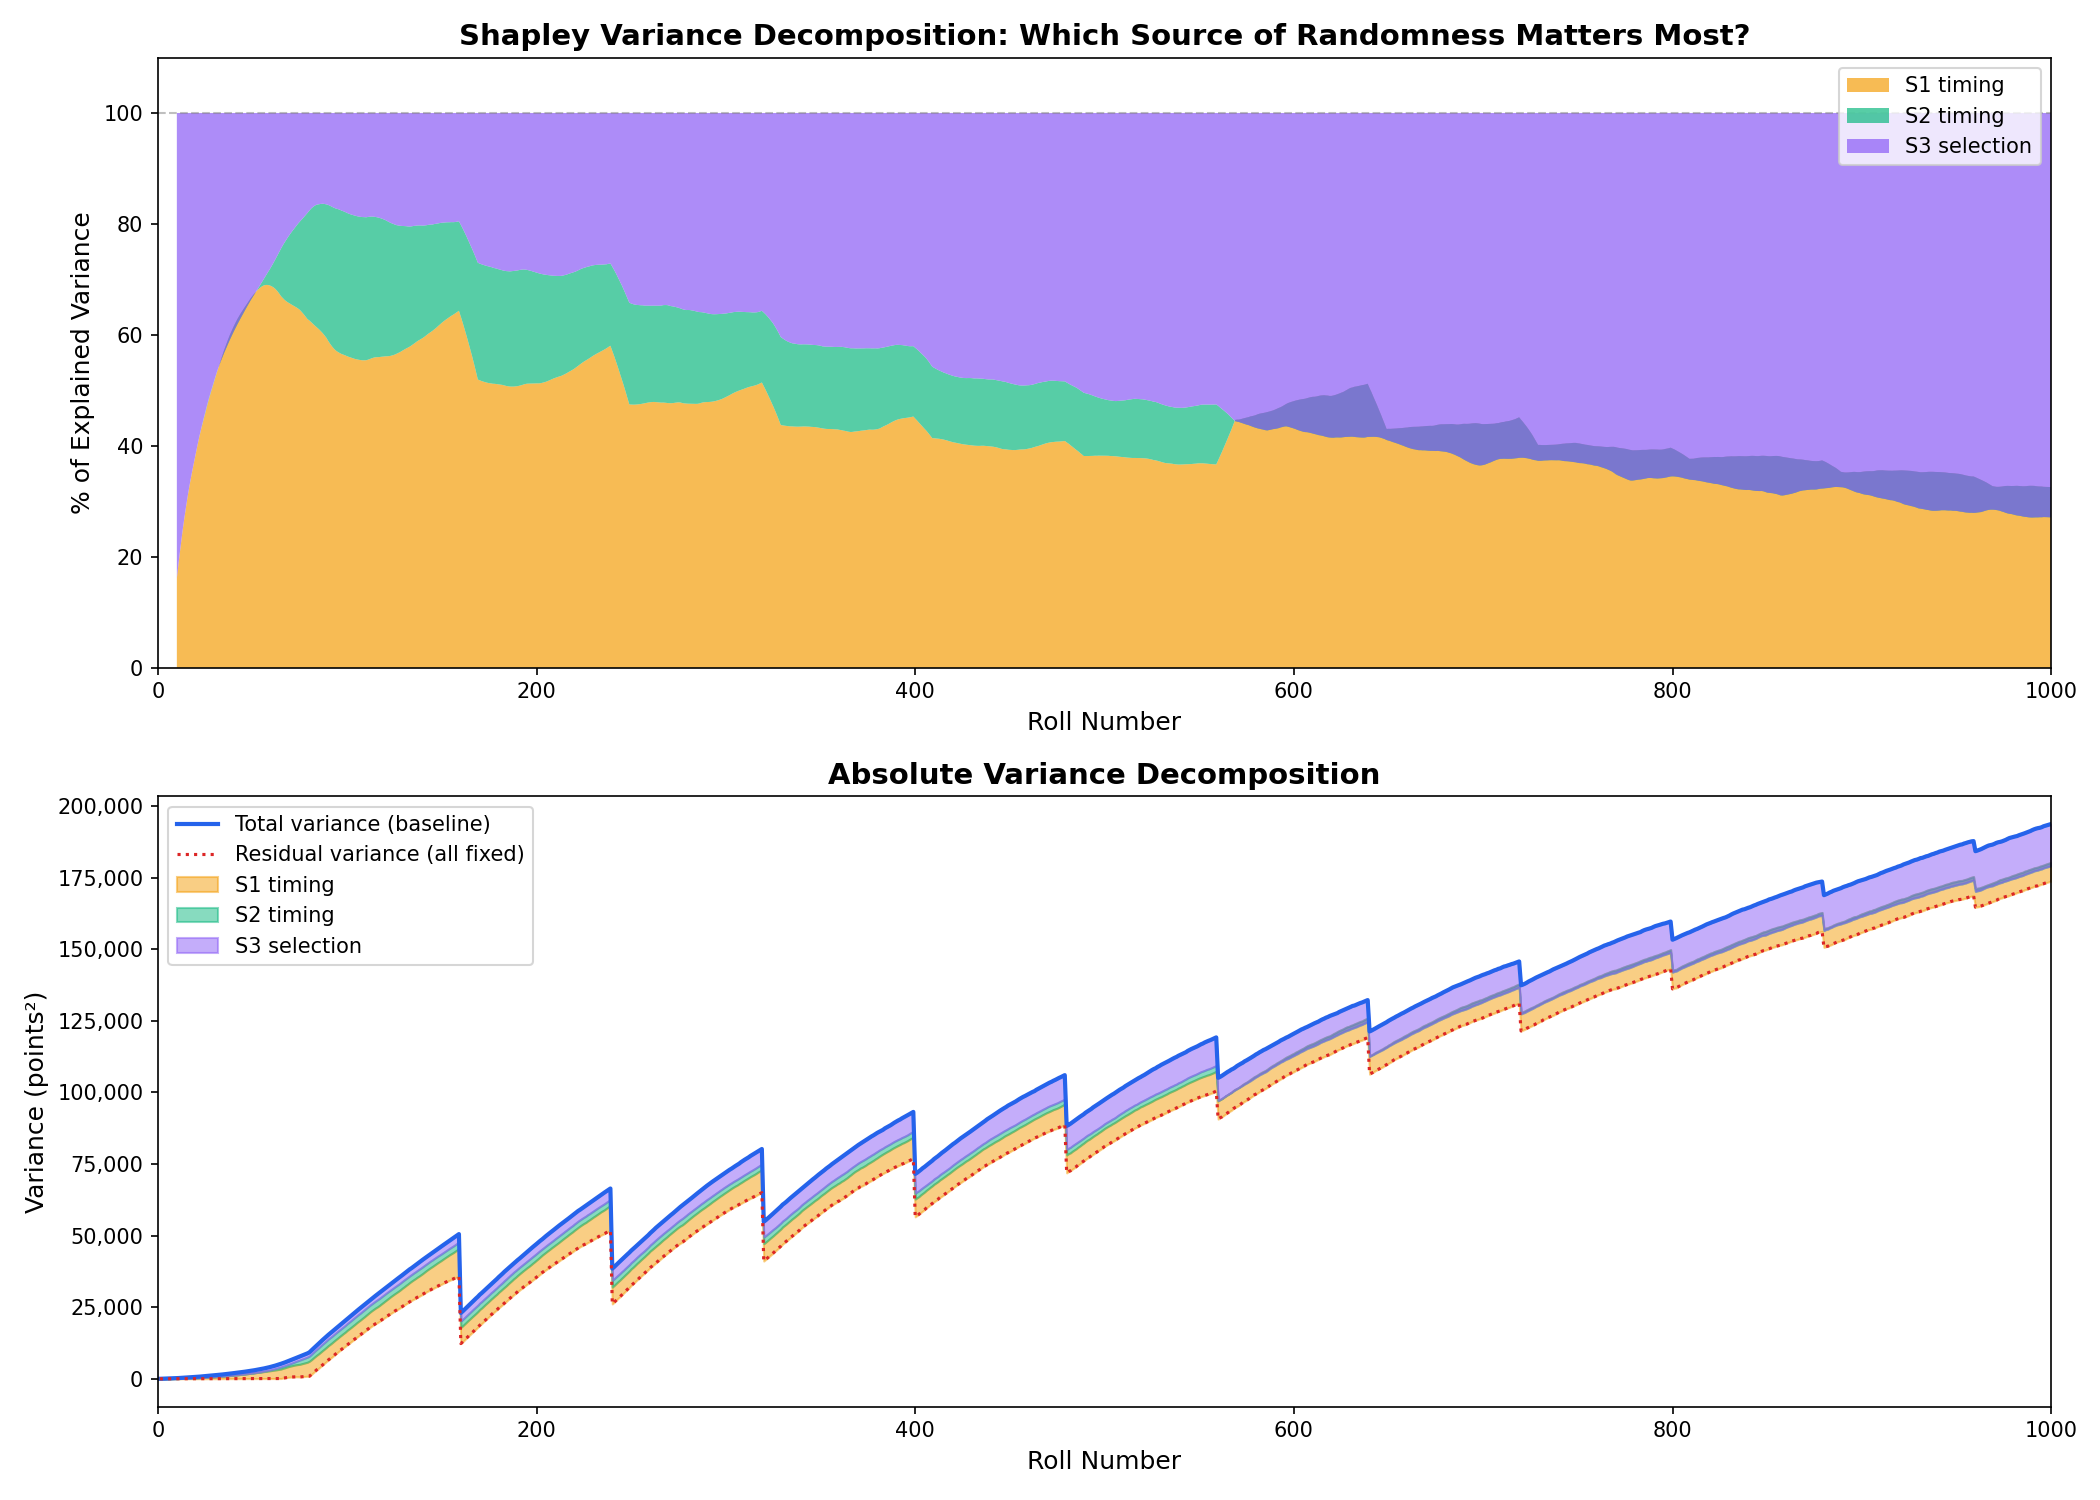
\includegraphics[width=\textwidth]{plots/variance_decomposition.png}
%     \caption{Shapley variance shares by roll. S1 timing dominates
%     the early-to-mid session before giving way to S3 selection noise
%     at higher roll counts.}
%     \label{fig:variance-decomp}
% \end{figure}


\subsection{Pity Cap Sweep: Point Accumulation and Cost}
\label{sec:results-sweep}

Table~\ref{tab:checkpoints} summarises mean cumulative points at key
checkpoints across all pity cap values.

\begin{table}[H]
\centering
\caption{Mean cumulative points at selected checkpoints by S1 pity
cap. All values from 300{,}000 simulations.}
\label{tab:checkpoints}
\begin{tabular}{r r r r r r r}
\toprule
Cap & Roll 10 & Roll 20 & Roll 30 & Roll 50 & Roll 80 & Roll 100 \\
\midrule
10 & 39.7  & 346.5 & 653.8  & 1{,}270.3 & 2{,}249.9 & 2{,}965.5 \\
20 & 42.3  & 81.3  & 146.8  & 508.4     & 1{,}197.8 & 1{,}651.7 \\
30 & 42.3  & 84.6  & 123.9  & 254.7     & 734.8     & 1{,}166.6 \\
40 & 42.3  & 84.6  & 127.4  & 232.7     & 673.8     & 924.1     \\
50 & 42.3  & 84.6  & 127.4  & 212.3     & 472.7     & 866.8     \\
60 & 42.3  & 84.6  & 127.4  & 215.8     & 452.5     & 683.4     \\
70 & 42.3  & 84.6  & 127.4  & 215.8     & 433.5     & 663.8     \\
80 & 42.3  & 84.6  & 127.4  & 215.8     & 414.8     & 645.2     \\
\bottomrule
\end{tabular}
\end{table}

\noindent Players fall into two broad categories. \emph{Skin-seekers}
enter the system aiming for the S1 max prize (the Viego skin),
which requires reaching the pity cap at roll~80 --- a cost of
\pounds213.98 using an optimal package combination.
\emph{Casual players} engage without committing to the full pity
distance and typically accumulate around 150 expected points
(roll~$\sim$38, \pounds102.49) before stopping. The gap between
these two endpoints --- \pounds111.49 --- defines the
\emph{sunk-cost trap} for casual players who did not initially
intend to reach pity but find themselves anchored by prior spend.

Table~\ref{tab:rolls-to-target} shows median rolls to reach point
milestones, with GBP equivalents.

\begin{table}[H]
\centering
\caption{Median rolls to reach point targets, with DP-optimal purchase cost.}
\label{tab:rolls-to-target}
\begin{tabular}{r r r r r r r}
\toprule
Cap & 50\,pts & 100\,pts & 150\,pts & 200\,pts & 300\,pts & 500\,pts \\
\midrule
10 & 14 (\pounds40)  & 20 (\pounds58)  & 20 (\pounds58)   & 20 (\pounds58)   & 20 (\pounds58)   & 30 (\pounds85)  \\
20 & 13 (\pounds39)  & 26 (\pounds74)  & 38 (\pounds102)  & 40 (\pounds108)  & 40 (\pounds108)  & 56 (\pounds152) \\
30 & 13 (\pounds39)  & 25 (\pounds71)  & 38 (\pounds102)  & 49 (\pounds133)  & 60 (\pounds164)  & 60 (\pounds164) \\
40 & 13 (\pounds39)  & 25 (\pounds71)  & 38 (\pounds102)  & 50 (\pounds134)  & 67 (\pounds178)  & 80 (\pounds214) \\
80 & 13 (\pounds39)  & 25 (\pounds71)  & 38 (\pounds102)  & 50 (\pounds134)  & 68 (\pounds182)  & 91 (\pounds244) \\
\bottomrule
\end{tabular}
\end{table}

\noindent A key observation: at the 150-point milestone, median rolls
are \emph{identical} across caps 20--80. For casual players, the cap
does not materially change how quickly they reach this point. For
skin-seekers, however, the cap \emph{is} the target: the pity
guarantee at roll~80 is the entire reason they are spending. The
cap determines both the cost of entry and the length of the
uncertainty they must endure to reach it.

% --- Figure: Mean points by cap ---
% \begin{figure}[H]
%     \centering
%     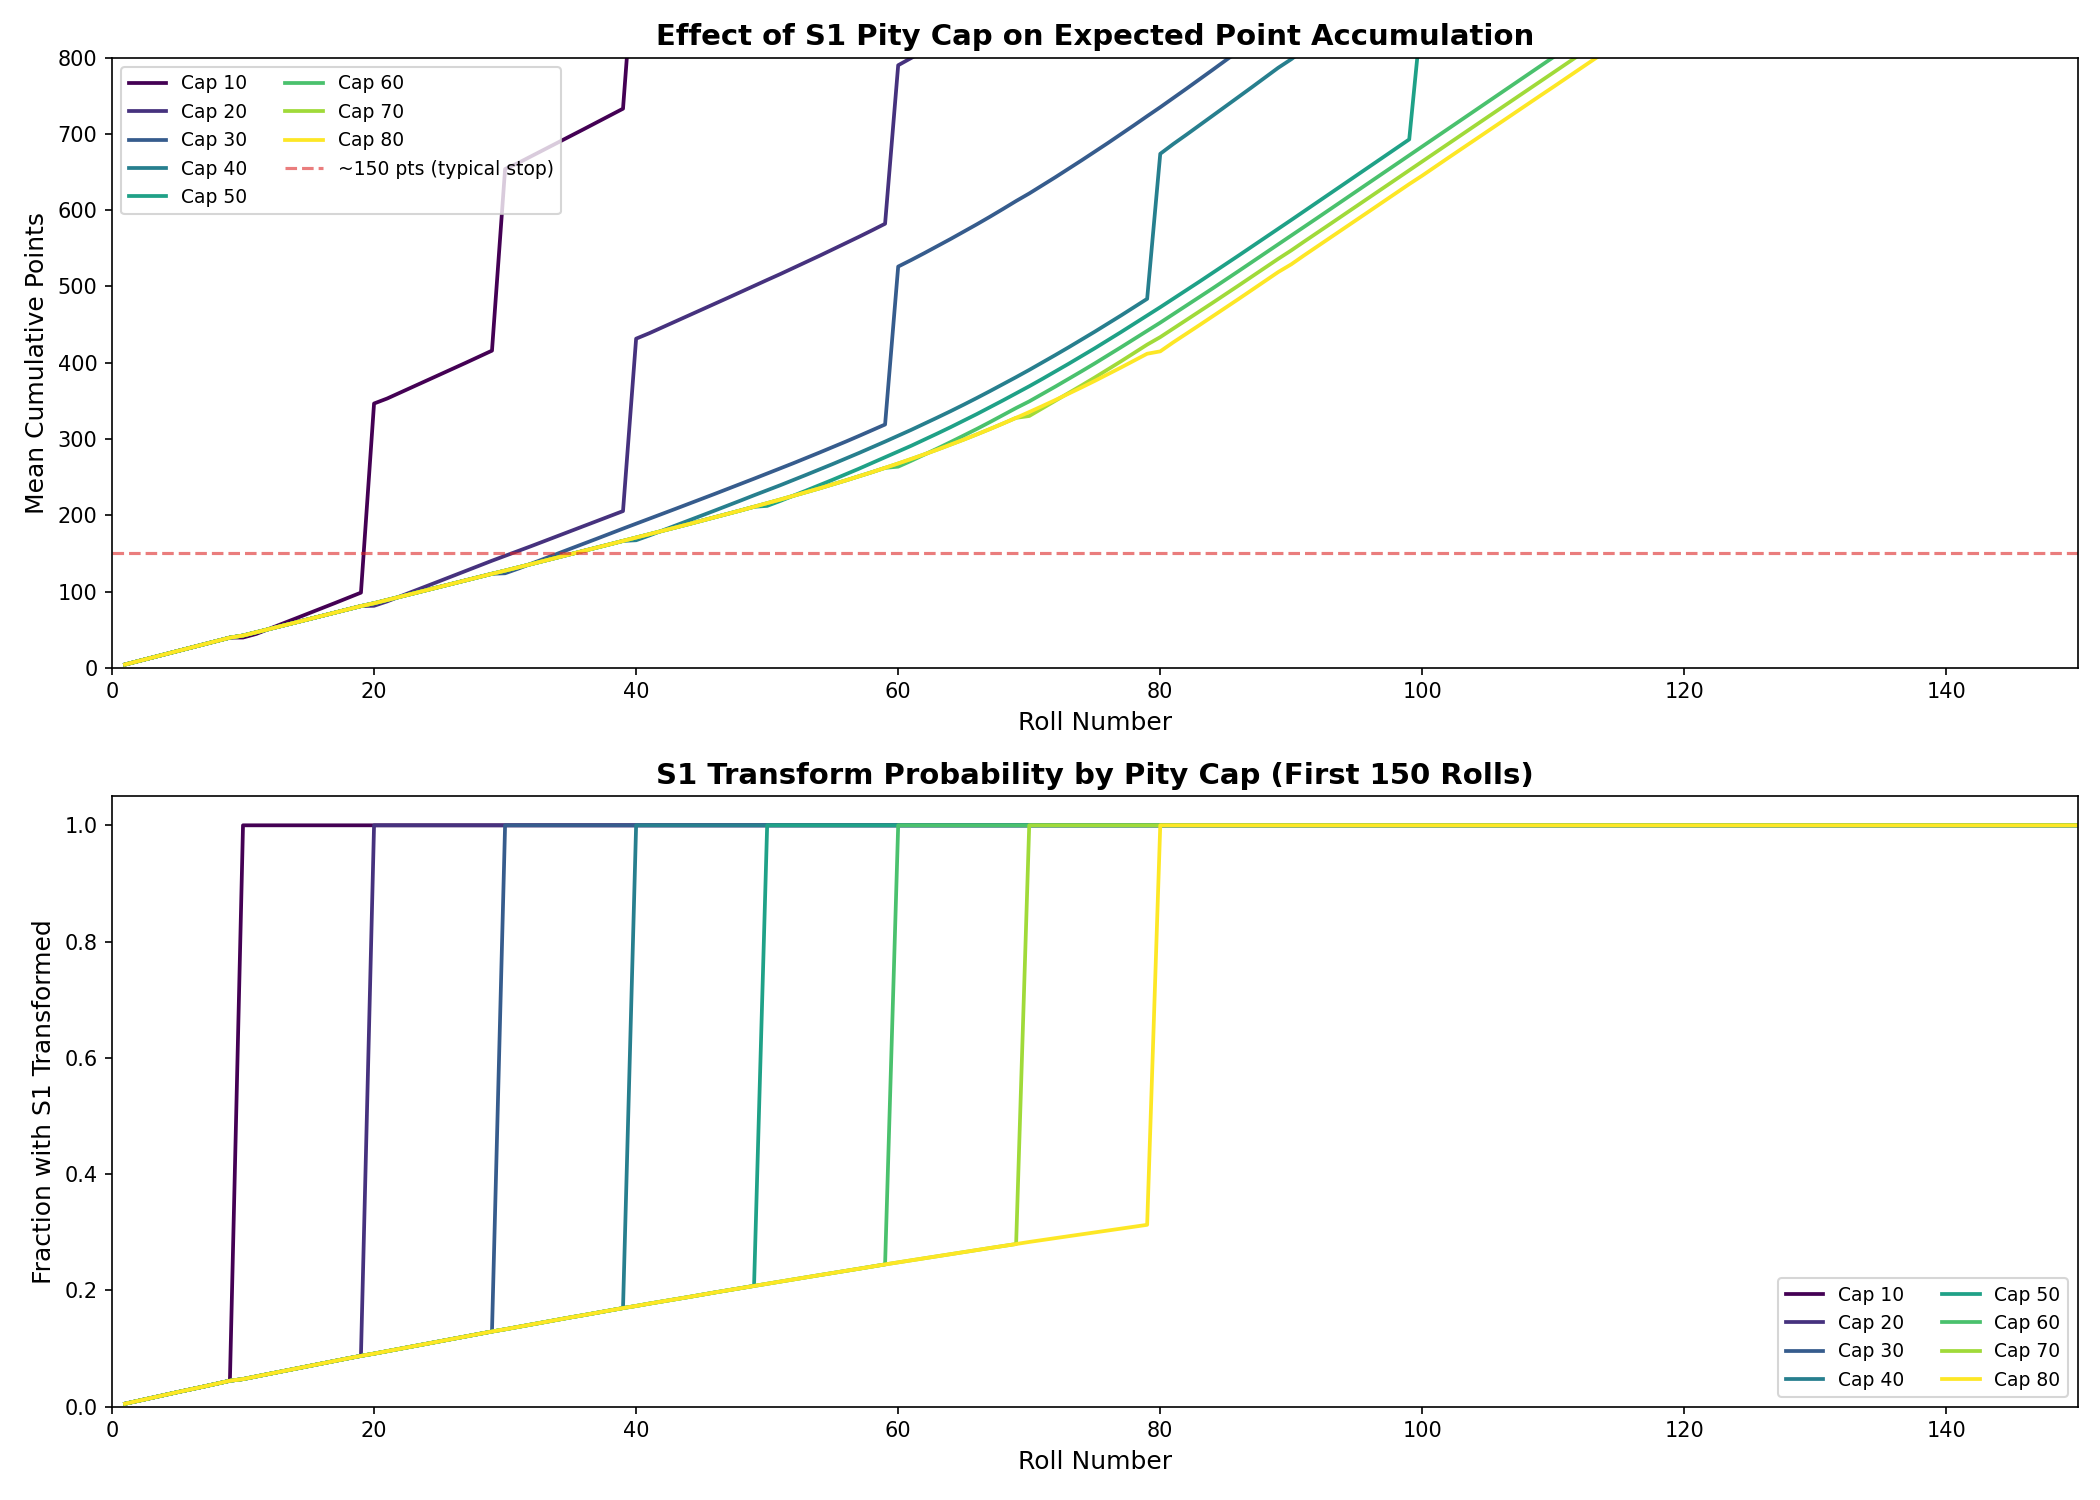
\includegraphics[width=\textwidth]{plots/pity_cap_mean_points.png}
%     \caption{Top: mean cumulative points vs roll number for each pity
%     cap. Bottom: fraction of simulations with S1 triggered. Lower caps
%     accelerate both point accumulation and S1 resolution.}
%     \label{fig:mean-points}
% \end{figure}

% --- Figure: Rolls to target ---
% \begin{figure}[H]
%     \centering
%     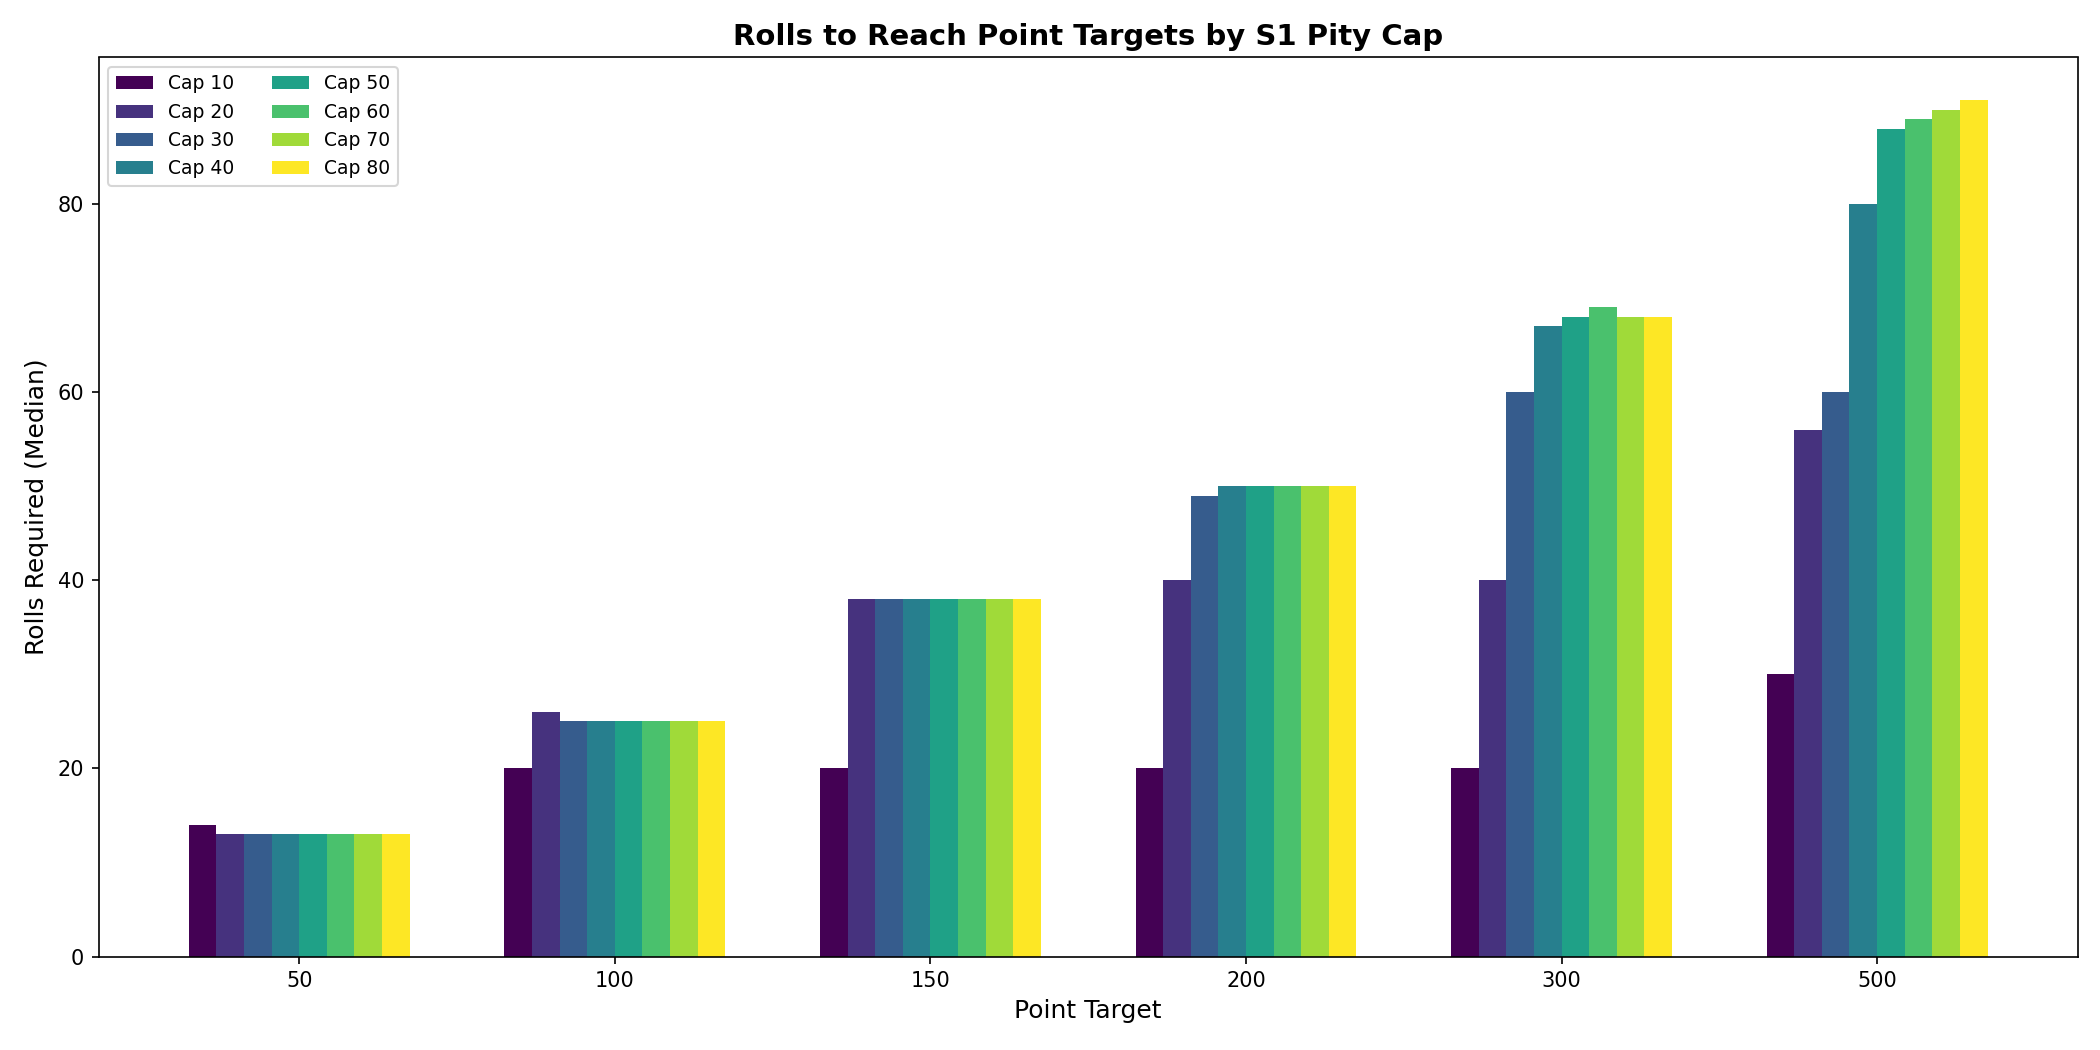
\includegraphics[width=\textwidth]{plots/pity_cap_rolls_to_target.png}
%     \caption{Median rolls required to reach point targets, grouped by
%     pity cap. Differences are negligible at low targets and widen
%     substantially at higher targets.}
%     \label{fig:rolls-target}
% \end{figure}


\subsection{The Uncertainty Window}
\label{sec:results-window}

Combining the variance decomposition with the pity cap sweep produces
the central result. Table~\ref{tab:uncertainty} shows the uncertainty
window --- the roll range where S1 timing drives more than 30\% of
total variance --- at each cap.

\begin{table}[H]
\centering
\caption{Uncertainty window by pity cap. Width is the number of rolls
where S1 timing accounts for $>$30\% of total outcome variance.}
\label{tab:uncertainty}
\begin{tabular}{r r r r r r}
\toprule
Cap & Median S1 & Start & End & Width & Peak share \\
\midrule
10 & 10 & ---  & ---  & 0  & 14.6\% \\
20 & 20 & 18   & 23   & 6  & 35.1\% \\
30 & 30 & 18   & 37   & 20 & 49.6\% \\
40 & 40 & 18   & 49   & 32 & 58.3\% \\
50 & 50 & 18   & 60   & 43 & 64.3\% \\
60 & 60 & 18   & 72   & 55 & 66.2\% \\
70 & 70 & 18   & 83   & 66 & 66.1\% \\
80 & 80 & 18   & 96   & 79 & 66.1\% \\
\bottomrule
\end{tabular}
\end{table}

\noindent At cap~80, the uncertainty window spans rolls 18--96. For
casual players (rolls 1--38), the entire session falls within this
zone. For skin-seekers (rolls 1--80), they spend their entire
journey inside the region of maximum outcome uncertainty before the
pity guarantee resolves it at the last possible moment.

Each 10-roll cap increment extends the window by 11--14 rolls:

\begin{table}[H]
\centering
\caption{Marginal impact of each 10-roll cap increase on the
uncertainty window, with DP-optimal purchase cost for those extra rolls.}
\label{tab:marginal}
\begin{tabular}{r r r r r}
\toprule
Change & Old width & New width & $\Delta$ rolls &
Extra spend (\pounds) \\
\midrule
$10 \to 20$ & 0  & 6  & $+6$  & 19.25 \\
$20 \to 30$ & 6  & 20 & $+14$ & 39.98 \\
$30 \to 40$ & 20 & 32 & $+12$ & 36.00 \\
$40 \to 50$ & 32 & 43 & $+11$ & 31.50 \\
$50 \to 60$ & 43 & 55 & $+12$ & 36.00 \\
$60 \to 70$ & 55 & 66 & $+11$ & 31.50 \\
$70 \to 80$ & 66 & 79 & $+13$ & 39.24 \\
\midrule
\textbf{Total} & & & \textbf{$+79$} &
\textbf{212.72} \\
\bottomrule
\end{tabular}
\end{table}

\noindent No single increment exceeds 14 rolls. Each change, viewed
in isolation, appears modest. The cumulative effect is an expansion
of 79 anxious rolls representing \pounds212.72 in potential additional
spend per player.

% --- Figure: Variance share by cap ---
% \begin{figure}[H]
%     \centering
%     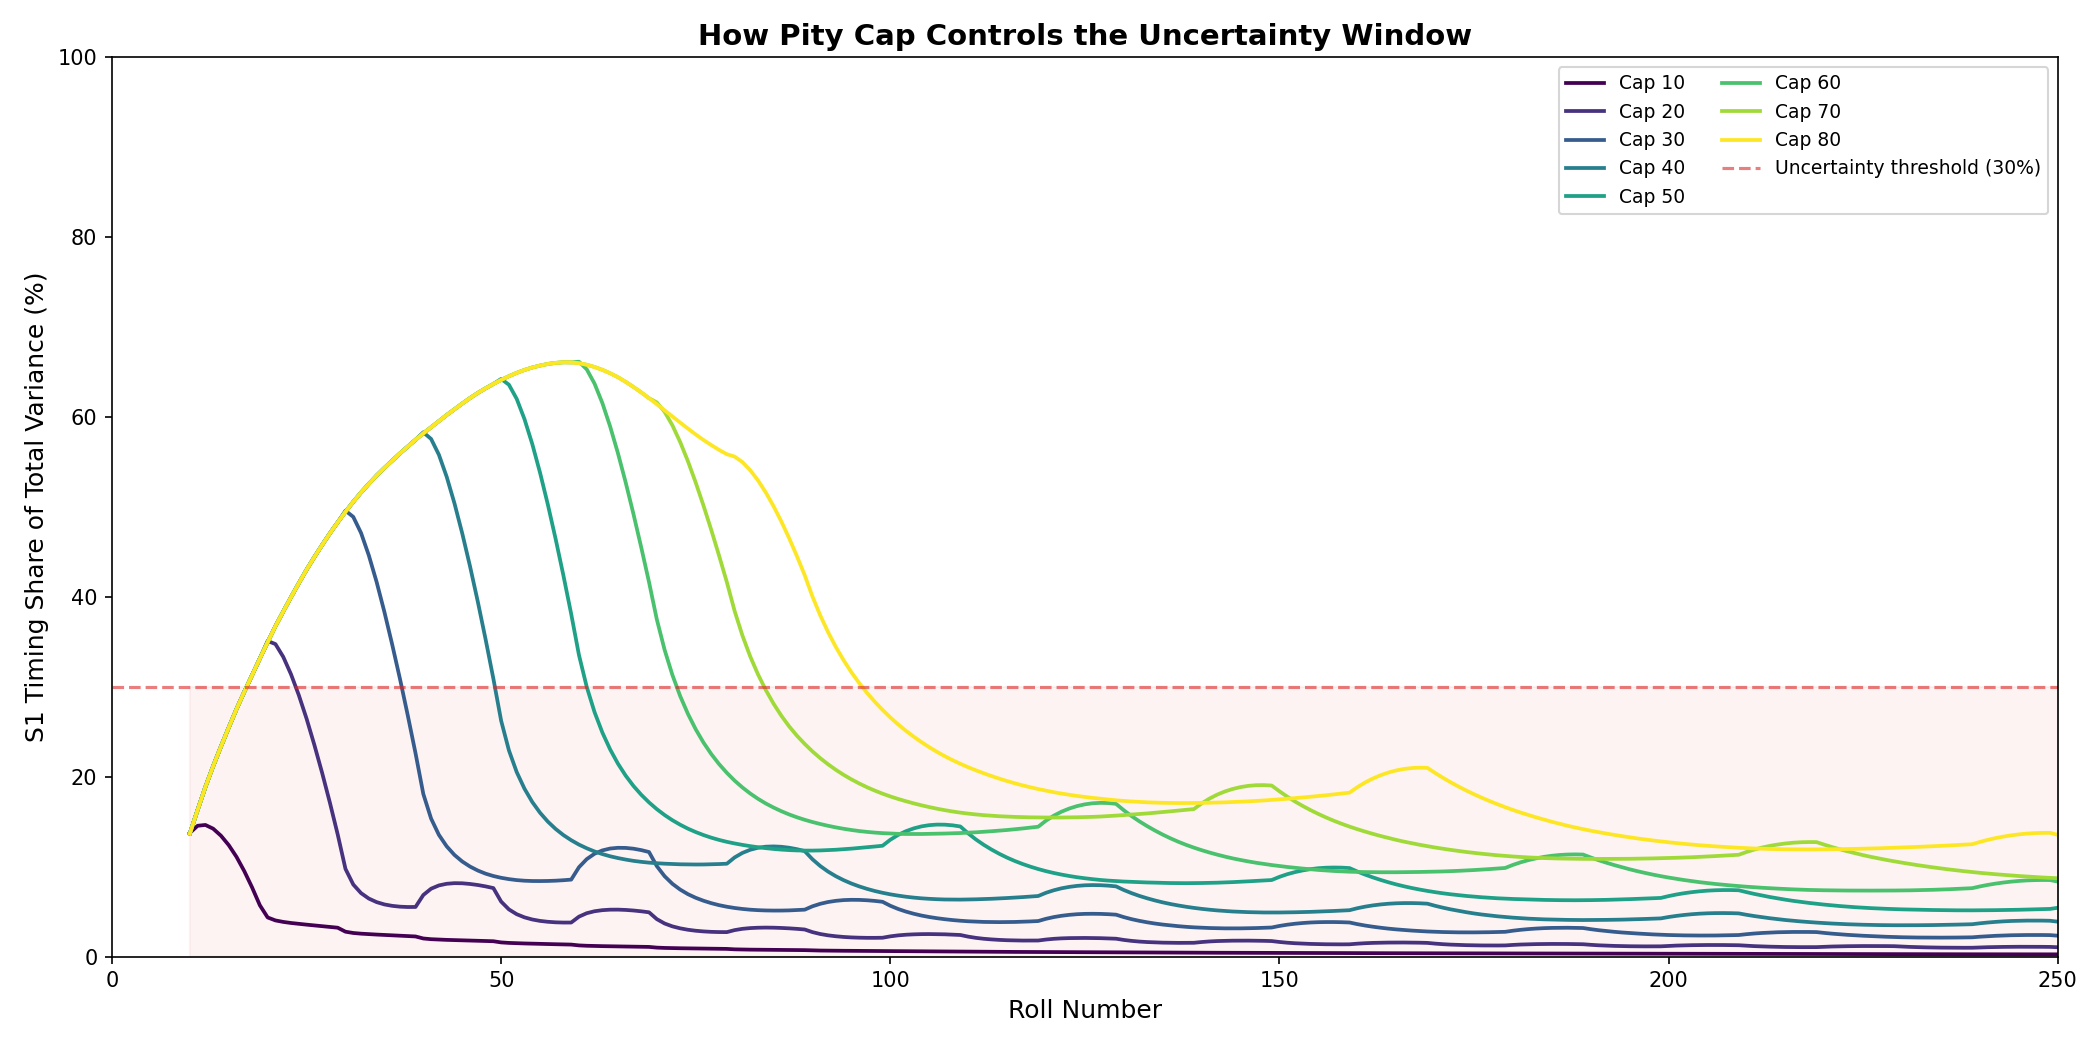
\includegraphics[width=\textwidth]{plots/synthesis_variance_share.png}
%     \caption{S1 variance share over roll number for each pity cap.
%     The dashed red line marks the 30\% uncertainty threshold. Higher
%     caps push the curve above this threshold for longer, widening the
%     uncertainty window.}
%     \label{fig:variance-share}
% \end{figure}

% --- Figure: Combined uncertainty + points (cap 80 vs 40) ---
% \begin{figure}[H]
%     \centering
%     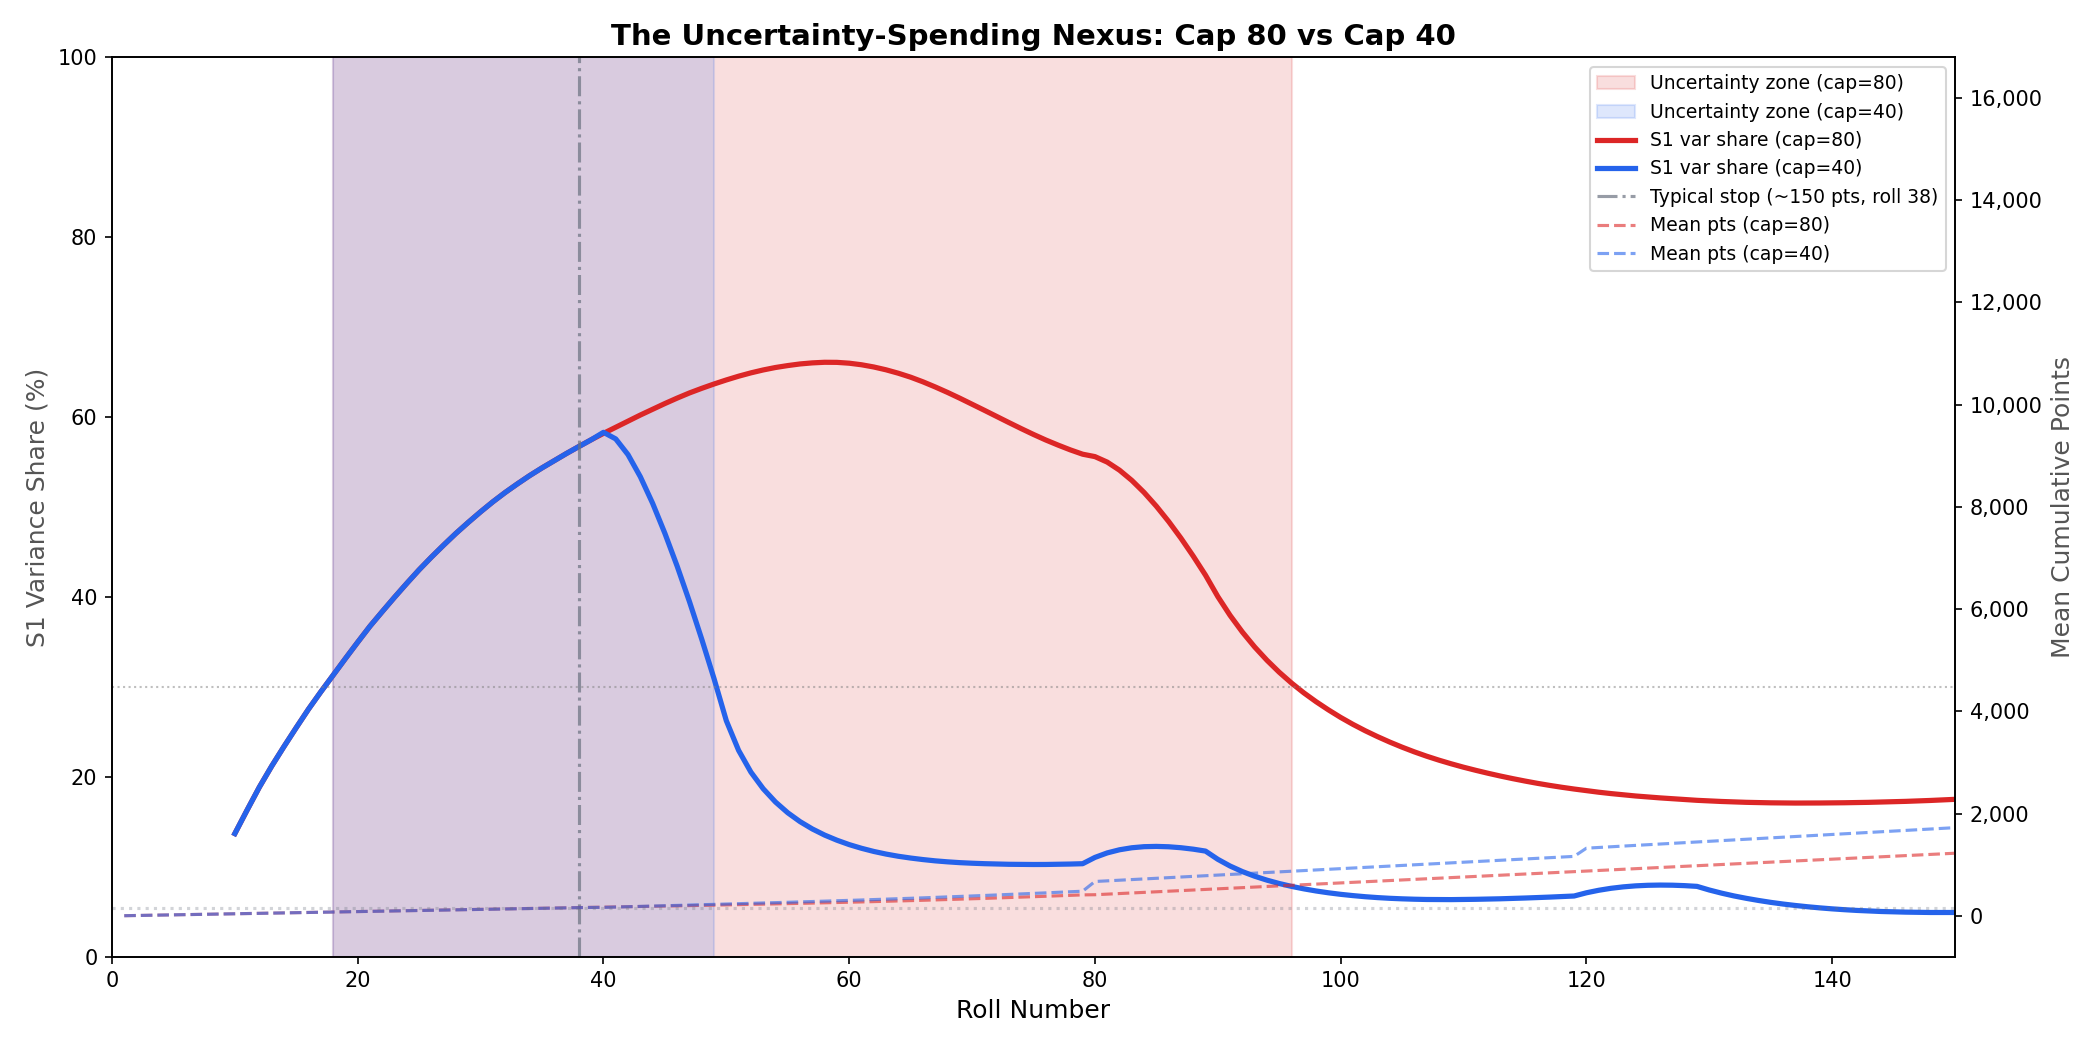
\includegraphics[width=\textwidth]{plots/synthesis_combined.png}
%     \caption{The uncertainty--spending nexus. Shaded regions show the
%     uncertainty window for cap~80 (red) and cap~40 (blue). The
%     vertical dashed line marks the typical stopping roll. At cap~80
%     the entire session falls within the anxious zone.}
%     \label{fig:combined}
% \end{figure}

% --- Figure: Marginal anxious rolls ---
% \begin{figure}[H]
%     \centering
%     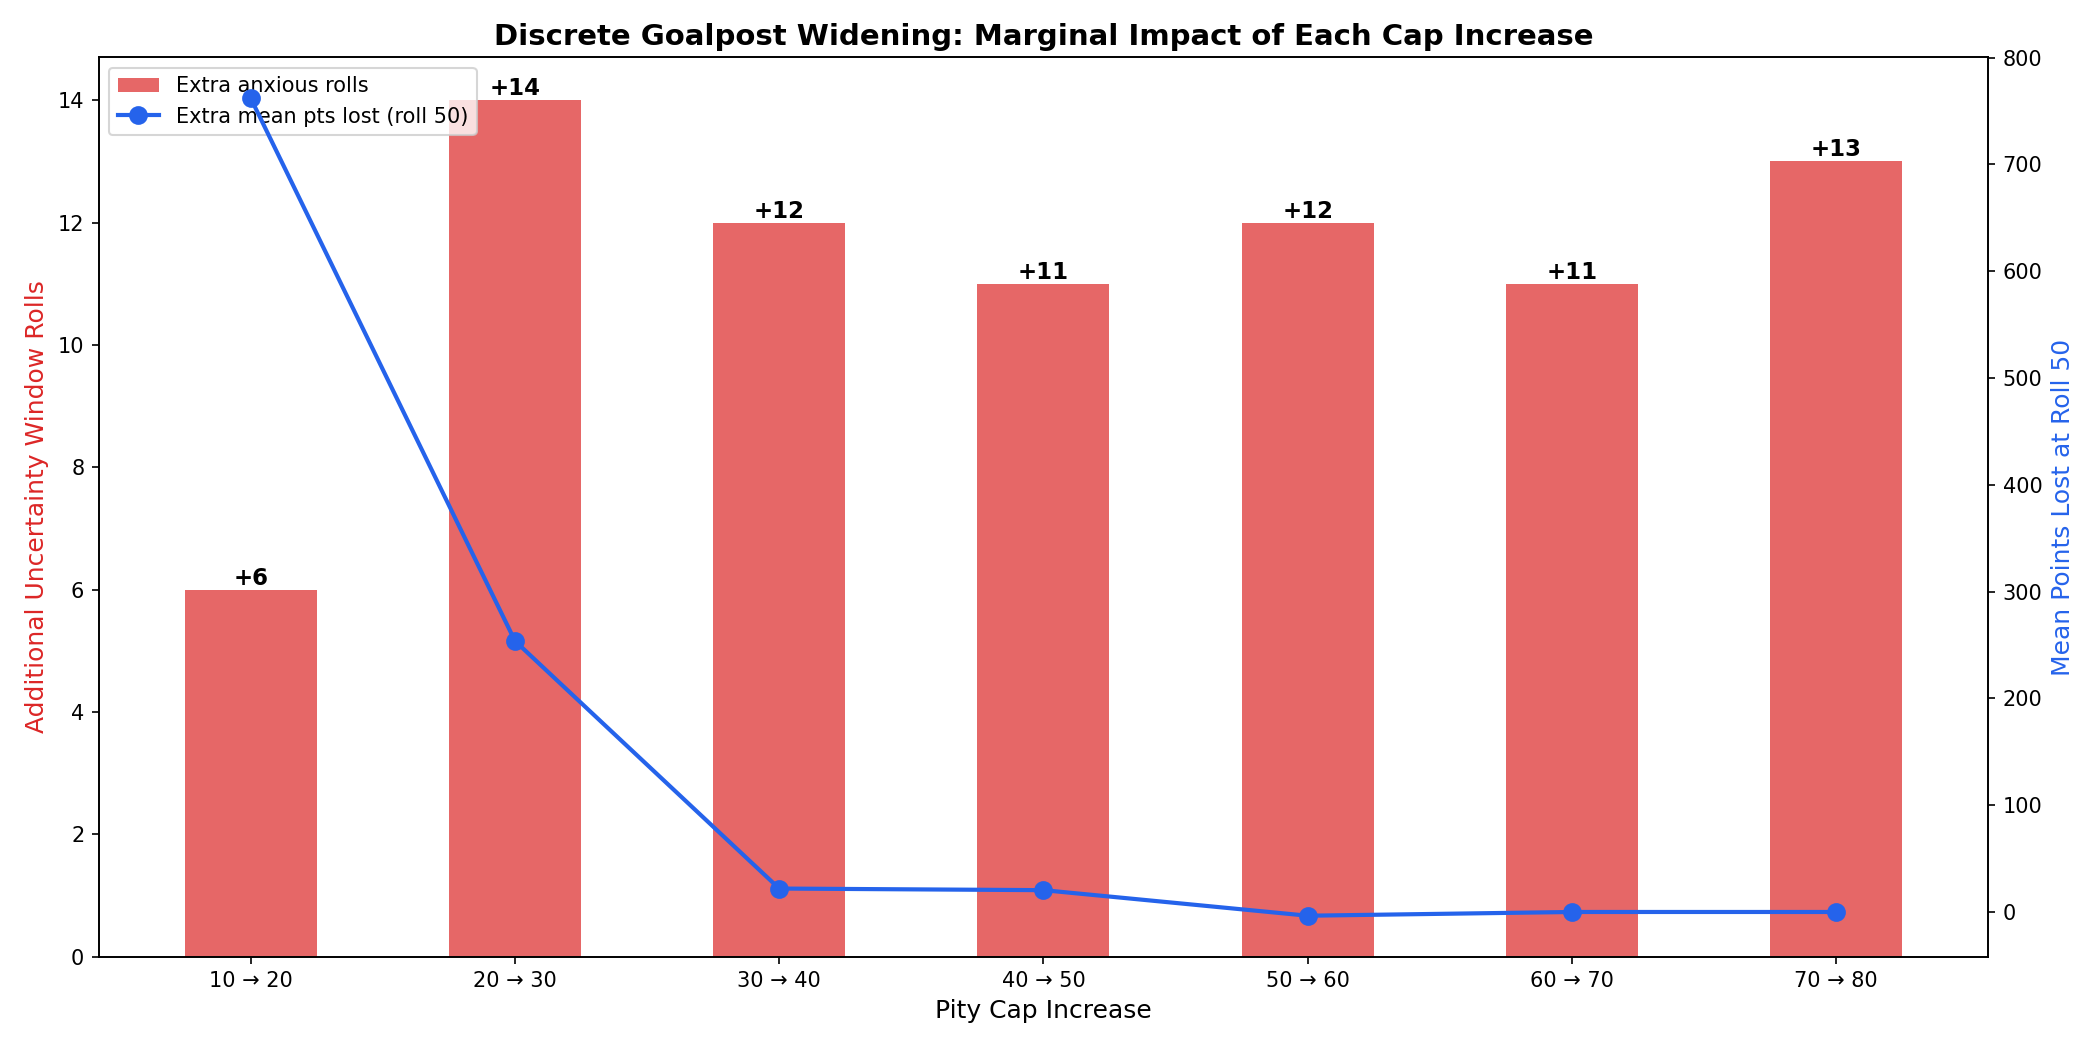
\includegraphics[width=\textwidth]{plots/synthesis_marginal_anxious.png}
%     \caption{Marginal expansion of the uncertainty window per 10-roll
%     cap increase (bars), overlaid with the corresponding loss in mean
%     points at the reference roll (line). Each increment is modest;
%     the cumulative effect is not.}
%     \label{fig:marginal-anxious}
% \end{figure}


% ======================================================================
\section{Synthesis: The Discrete Goalpost Widening Effect}
\label{sec:synthesis}
% ======================================================================

The results converge on a single mechanism, described here in three
parts.

\subsection{The Monetisation Geometry}
\label{sec:synthesis-geometry}

At 400~RP per roll, using optimal package combinations, two
distinct spending trajectories emerge:

\begin{itemize}[nosep]
    \item \textbf{Skin-seekers} target the S1 pity guarantee and
          budget for roll~80: \pounds213.98. This is their
          \emph{intended} spend from the outset.
    \item \textbf{Casual players} accumulate $\sim$150 points by
          roll~$\sim$38: \pounds102.49. At this threshold the
          accumulated points can be redeemed for a specific reward
          outside the loot system, providing a natural exit point.
    \item The gap between these endpoints: \pounds111.49.
\end{itemize}

For \textbf{casual players}, the gap is the monetisation sweet spot:
large enough to extract significant additional spend, but framed as
``finishing what you started'' rather than initiating a new purchase.
At roll~38 with cap~80, only 16.5\% of players have triggered S1.
Those who stop here leave without the max prize, and the pity cap
functions as a \emph{psychological anchor} --- a visible guarantee
that reframes quitting as a loss.

For \textbf{skin-seekers}, the monetisation operates differently.
These players enter the system already committed to reaching the
pity cap. The uncertainty window does not need to \emph{trick} them
into spending more --- they have already accepted the full cost. Instead,
the cap's function is to \emph{set the price}: an 80-roll cap means
\pounds214 rather than the \pounds85--\pounds108 it would cost at
caps of 30--40. The discrete goalpost widening effect determines
\emph{how much} the skin costs, not whether the player pursues it.
A player who would have paid \pounds85 for the skin at cap~30 must
now pay \pounds214 for the identical outcome at cap~80.


\subsection{Package Granularity and Forced Overspend}
\label{sec:synthesis-packages}

The spending pressure created by the pity cap does not operate in
isolation --- it is compounded by the structure of the RP package
store. Table~\ref{tab:packages} lists the available packages.

\begin{table}[H]
\centering
\caption{RP packages with effective rolls per package. Only the
2{,}800~RP package yields a whole number of rolls (400~RP each).}
\label{tab:packages}
\begin{tabular}{r r r r}
\toprule
RP & GBP & Rolls covered & GBP/roll \\
\midrule
575      & \pounds4.50   & 1.44  & \pounds3.13 \\
1{,}380  & \pounds10.25  & 3.45  & \pounds2.97 \\
2{,}800  & \pounds19.99  & 7.00  & \pounds2.86 \\
4{,}500  & \pounds31.50  & 11.25 & \pounds2.80 \\
6{,}500  & \pounds44.99  & 16.25 & \pounds2.77 \\
13{,}500 & \pounds88.99  & 33.75 & \pounds2.64 \\
33{,}500 & \pounds220.00 & 83.75 & \pounds2.63 \\
60{,}200 & \pounds385.00 & 150.50 & \pounds2.56 \\
\bottomrule
\end{tabular}
\end{table}

\noindent Two properties of this structure deserve attention.

\subsubsection*{1. Fractional Roll Counts}

Most packages yield a fractional number of rolls. Only the 2{,}800~RP
package divides cleanly (7.00 rolls exactly). All others produce a
fractional remainder, meaning that \emph{no single purchase of those
packages} can be exactly exhausted through rolling --- there is always
a residual RP balance.

Even with an optimal combination chosen by the DP algorithm, achieving
a specific roll target still requires overspending slightly. Consider
both player types:

\textbf{Casual player} targeting 150 points ($\sim$38 rolls =
15{,}200~RP):

\begin{itemize}[nosep]
    \item Optimal combination: $1 \times 13{,}500$ RP (\pounds88.99)
          $+ 3 \times 575$ RP (\pounds13.50) = 15{,}225~RP ---
          25~RP surplus --- total \pounds102.49.
    \item Alternative: $1 \times 13{,}500 + 1 \times 1{,}380 +
          1 \times 575$ RP (\pounds103.74): yields 15{,}455~RP ---
          255~RP surplus, \pounds1.25 more expensive.
\end{itemize}

\textbf{Skin-seeker} targeting the pity cap (80 rolls = 32{,}000~RP):

\begin{itemize}[nosep]
    \item Optimal combination: $2 \times 13{,}500$ RP (\pounds177.98)
          $+ 1 \times 4{,}500$ RP (\pounds31.50) $+ 1 \times 575$ RP
          (\pounds4.50) = 32{,}075~RP --- 75~RP surplus ---
          total \pounds213.98.
    \item Alternative: $1 \times 33{,}500$ RP (\pounds220.00):
          yields 33{,}500~RP --- 1{,}500~RP (3.75 rolls) surplus,
          \pounds6.02 more expensive.
\end{itemize}

\noindent Even the optimal purchase produces residual RP --- a
\emph{re-engagement hook} that feels wasteful to abandon. The casual
player's 25~RP surplus and the skin-seeker's 75~RP surplus are each
insufficient for even one additional roll (which costs 400~RP), yet
both create a balance that nudges toward a further top-up purchase.

\subsubsection*{2. Non-Uniform Increments}

The package sizes (575, 1{,}380, 2{,}800, 4{,}500, 6{,}500,
13{,}500, 33{,}500, 60{,}200) are not multiples of a common base.
If packages were sold in clean multiples of 400~RP, a player could
calculate exactly how many rolls they were buying and purchase
accordingly. Instead, the irregular increments introduce a
\emph{currency obfuscation layer}: the conversion from pounds to RP
to rolls requires mental arithmetic that most players will
approximate rather than compute precisely.

This approximation systematically favours the house. A player who
reasons ``the 13{,}500~RP package should cover 38 rolls'' is
200~RP short (13{,}500 $<$ 15{,}200). A player who guesses
``two 6{,}500~RP packages'' has 13{,}000~RP --- still 2{,}200~RP
short of 38 rolls. In both cases, the player either stops short of
their target or buys an additional package, generating surplus RP
that seeds further spending.

\subsubsection*{Interaction with the Pity Cap}

The package structure and the pity cap form a complementary system.
The pity cap determines \emph{how many rolls} a player desires by
anchoring a guaranteed outcome at a specific distance. The package
structure ensures that \emph{purchasing those rolls} always involves
waste. Together, they create a two-layer extraction mechanism:

\begin{enumerate}[nosep]
    \item The uncertainty window pressures the player to want more
          rolls than they originally intended.
    \item The package granularity ensures that buying those rolls
          produces leftover currency that encourages yet another
          session.
\end{enumerate}

\noindent This interaction means that the real cost of engaging with
the system always involves some overspend beyond the exact RP
required. Even with optimal package selection, the casual player
pays \pounds102.49 for 15{,}225~RP when they need 15{,}200~RP, and
the skin-seeker pays \pounds213.98 for 32{,}075~RP when they need
32{,}000~RP. In both cases, residual RP either goes unused or seeds
further spending.


\subsection{Three Psychological Functions of the Pity Cap}
\label{sec:synthesis-psychology}

\subsubsection*{1. Sunk Cost Anchor}

For \textbf{casual players}, reaching 150 points (roll~38) creates
a framing where they are 42 rolls away from a guaranteed outcome.
Stopping is reframed as a \emph{loss} --- walking away from a
``sure thing'' --- rather than a natural endpoint. The gap
represents \pounds111.49 of additional spend at optimal pricing.

For \textbf{skin-seekers}, the sunk cost operates in reverse:
having committed to the \pounds213.98 spend from the start, they are
anchored to completing all 80 rolls regardless of intermediate
outcomes. A skin-seeker who triggers S1 naturally at roll~30 has
``wasted'' their remaining budget headroom, but a skin-seeker at
roll~60 without S1 has already spent \pounds164.22 and faces the
classic sunk-cost compulsion to continue.

\subsubsection*{2. Near-Miss Framing}

For \textbf{casual players}, with only 16.5\% triggering S1 by
roll~38, most leave feeling they ``almost'' got lucky. The variance
decomposition confirms this is not paranoia: S1 timing genuinely is
the dominant factor separating good outcomes from bad ones in the
early-to-mid session (68.9\% of explained variance at roll~50). A
lower cap would resolve this uncertainty earlier, collapsing the
emotional hook before it becomes entangled with spending decisions.

For \textbf{skin-seekers}, near-miss framing operates throughout
their entire session. Every roll that does not trigger S1 naturally
(at 0.5\% per roll) reinforces the feeling that the next roll
\emph{could} be the one --- even though the simulation shows the
median player never triggers S1 before the pity cap forces it.
The 79-roll uncertainty window means the skin-seeker spends their
entire journey in a state of manufactured near-miss anticipation.

\subsubsection*{3. Discrete Invisibility}

Each 10-roll cap increase adds only 11--14 anxious rolls. No single
change feels dramatic. A designer moving the cap from 40 to 50 adds
11 rolls of uncertainty --- approximately \pounds31.50 in potential
spend --- an increment that would be difficult for players to
perceive, let alone protest. But the cumulative effect from cap~10
to cap~80 is 79 extra anxious rolls worth \pounds212.72.

This is the core of the discrete goalpost widening effect: a series
of individually invisible adjustments that, in aggregate, reshape the
entire psychological landscape of a player's session.


\subsection{The Isolation Property}
\label{sec:synthesis-isolation}

The interaction effects from the $2^3$ factorial analysis deserve
emphasis. All S1$\times$S2, S1$\times$S3, S2$\times$S3, and
S1$\times$S2$\times$S3 interaction terms are below 1.5\% of
baseline variance at every checkpoint examined. This means that the
pity cap operates as an \emph{independent lever}: adjusting it does
not create cascading effects on S2 completion dynamics or S3 item
selection. From a system design perspective, this is a precision tool.
The designer can tune spending pressure with confidence that only the
intended variable is affected.


% ======================================================================
\section{What a Fairer System Would Look Like}
\label{sec:fair}
% ======================================================================

The analysis also reveals what the system \emph{could} be.

At a pity cap of 30, the uncertainty window spans rolls 18--37 with a
width of 20 rolls and a peak S1 variance share of 49.6\%. This places
the resolution of outcome uncertainty approximately at the 150-point
redemption threshold (roll~$\sim$38): by the time a casual player
reaches their exit point, the question of whether they were ``lucky''
has been substantially answered. For skin-seekers, a cap of 30 means
the max prize costs \pounds84.97 rather than \pounds213.98 --- the
guaranteed outcome is delivered within a spend comparable to what
casual players already accept.

At cap~40, the window is 32 rolls wide (rolls 18--49), still
resolving within a reasonable horizon. The cost to reach the pity
guarantee is \pounds108.24 --- comparable to the casual player's
spend at the 150-point threshold. Skin-seekers would pay roughly
what casual players already pay, rather than more than double.

Either of these configurations would preserve the consumer-facing
function of the pity mechanic (protection against extreme bad luck)
while substantially reducing its secondary function as a spending
pressure tool. Casual players would still experience uncertainty ---
this is inherent to any probabilistic system --- but that uncertainty
would not be \emph{architecturally extended} to coincide with every
spending decision they make during their session. Skin-seekers would
face a price proportional to the game's natural economy rather than
one inflated by 79 additional anxious rolls.


% ======================================================================
\section{Limitations}
\label{sec:limitations}
% ======================================================================

Several limitations should be noted.

First, the analysis identifies two player archetypes --- casual
players who exit at the 150-point redemption threshold and
skin-seekers who commit to the pity cap --- but real player
behaviour is a continuum. Some players stop before 150 points,
others fall between the two archetypes, and whale spending
patterns differ qualitatively. Modelling a distribution of player
types and their interaction with the uncertainty window would
strengthen the conclusions.

Second, the psychological mechanisms described --- sunk cost,
near-miss framing, discrete invisibility --- are inferred from the
statistical structure rather than measured directly through player
data or behavioural experiments. The simulation demonstrates that
the \emph{conditions} for these effects exist; it does not prove
that players experience them as described.

Third, the model treats each roll as an independent spending
decision. In practice, players purchase RP in discrete packages and
pre-commit to a batch of rolls. As shown in
Section~\ref{sec:synthesis-packages}, this does not weaken the
spending pressure argument --- the package granularity introduces a
second layer of extraction by forcing overspend and creating
residual balances. However, the analysis does not model how
\emph{package boundary decisions} (``do I buy another package?'')
interact with the uncertainty window. The psychological dynamics at
these discrete purchase points may differ from the continuous-roll
model assumed here.

Fourth, only the S1 pity cap is varied. The S2 pity system (not
explored here) introduces additional interactions that may modify the
overall spending pressure landscape at higher roll counts.


% ======================================================================
\section{Conclusion}
\label{sec:conclusion}
% ======================================================================

This analysis demonstrates that the S1 pity cap in the Sanctum loot
system functions as a monetisation lever with three convergent
properties:

\begin{enumerate}[nosep]
    \item \textbf{Variance dominance.} S1 timing accounts for up to
          68.9\% of explained outcome variance in the critical
          early-to-mid session. Whether a player's experience feels
          lucky or unlucky is overwhelmingly determined by a single
          binary event.

    \item \textbf{Window extension.} Each 10-roll increase in the
          pity cap extends the zone of peak uncertainty by 11--14
          rolls. At cap~80, this zone spans the player's entire
          natural session.

    \item \textbf{Clean isolation.} The pity cap operates independently
          of S2 and S3 dynamics, with all interaction effects below
          1.5\% of baseline variance. It is a precision instrument.
\end{enumerate}

The cumulative effect --- discrete goalpost widening --- transforms a
consumer protection mechanic into a spending optimisation tool that
operates on both player archetypes simultaneously. For casual players
(targeting the 150-point redemption threshold), the cap at 80 rolls
creates \pounds111.49 of sunk-cost distance beyond their exit point and
ensures that 83.5\% leave inside the uncertainty window. For
skin-seekers (targeting the max prize), the cap sets the price of
the guaranteed outcome at \pounds213.98 rather than the \pounds84.97--\pounds108.24
it would cost at caps of 30--40 --- a surcharge applied entirely
through the uncertainty window. In both cases, the extraction is
achieved through increments that are individually invisible.

The data suggests that a cap of 30--40 rolls would preserve the
protective function of the pity system while resolving outcome
uncertainty within the casual player's session and pricing the max
prize proportionally to the game's natural economy. The difference
between cap~40 and cap~80 is not player protection --- it is
\pounds105.74 of additional spending pressure per player, applied
through a mechanism that is statistically precise and psychologically
difficult to perceive.

\end{document}
